\section{Moving-Object Analysis}
\label{sec:processing}

The calibrated images and catalogs feed the two analysis paths shown in
Figure~\ref{fig:workflow}. Ephemeris association measures sources at
predicted asteroid positions. The independent search first seeks
consistent motion, then uses the known-object associations to remove
already attributed linkages. Both paths retain the connection between a
measurement, its exposure, and the corresponding image.

\begin{figure}[tbp]
\centering
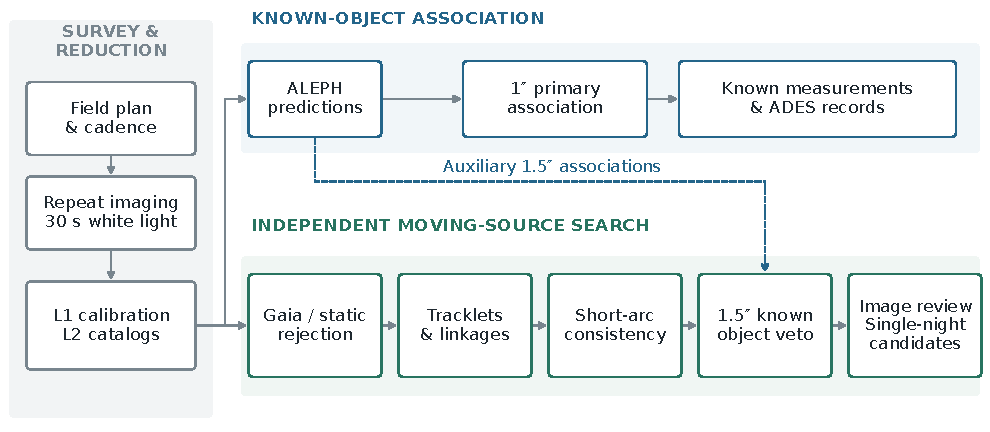
\includegraphics[width=\linewidth]{fig02_workflow.pdf}
\caption{The observing and analysis sequence used in the initial \SHARP\
campaign. Repeated white-light imaging produces calibrated L1 images
and L2 source catalogs. The upper branch associates measured sources
with ALEPH predictions and supplies the primary $1\asec$ known-object
sample. The independent moving-source branch constructs tracklets and
links after static-source rejection, tests short-arc consistency, and
then removes links identified through auxiliary $1.5\asec$ known-object
associations. The dashed connection supplies these identities after
moving-source linking. Image review selects the retained single-night
candidates.}
\label{fig:workflow}
\end{figure}

\label{sec:known_method}

For each exposure, the known-object branch evaluates topocentric asteroid
directions at the exposure midpoint using the archived Lowell
\texttt{astorb} orbital catalog \citep{Moskovitz2022Astorb} and
ALEPH version~1.0.0 \citep{PenaZamudioFuentes2021ALEPH}. The prediction uses the
Xinglong position adopted by the historical matcher:
$117.575^\circ$ east longitude, $40.393^\circ$ north latitude, and 960~m
height. We use this location consistently for the known-object
viewing geometry.

Predictions with $V<22.5$ that fall within the image geometry are compared
with measured sources. The primary catalog retains the nearest
association within $1.0\asec$; a separate $1.5\asec$ association table is
used for known-object subtraction and processing diagnostics. The
predicted magnitude limit defines the ephemeris query, rather than the
exposure detection limit. The historical matcher checks finite
photometric fields but does not impose a physically restrictive
consistency cut between predicted $V$ and measured \gaper. This matters
particularly for sparse associations to objects in less populated
orbital regions.

The prediction catalog contains asteroid orbital elements. Comets were
therefore outside the contemporaneous known-object subtraction, a point
relevant to the C/2025~Y1 associations discussed in
Section~\ref{sec:candidates}. Selected measurements are also stored in
Astrometric Data Exchange Standard (ADES) format.

\label{sec:motion_method}

The independent search starts from detections in repeated catalogs of a
field. Gaia associations, stationary-source patterns, and edge-related
detections are removed before constructing two-detection tracklets.
Tracklets sharing endpoints can be combined into links with at least
three measurements. The historical search accepts angular rates of
$3$--$63$~\rateunit, a magnitude difference no larger than 1~mag within
a tracklet, a tracklet-rate difference no larger than
5~\rateunit, and a direction difference no larger than $10^\circ$.
These criteria define the initial search window and help suppress
inconsistent combinations of detections.

A heliocentric short-arc calculation then tests whether a candidate chain
admits a consistent trajectory. Heliocentric transformations are useful
for linking moving-source observations \citep{Holman2018}; the
implementation used here evaluates the within-night chains generated by
the preceding tracklet step. A successful short-arc fit and the absence
of auxiliary known-asteroid associations for all members define the
historical automatic candidate catalog. All 4,762 selected links also satisfy the separately evaluated
diagnostic thresholds: fit RMS $\leq5\asec$, maximum residual
$\leq8\asec$, and linear-trajectory RMS $\leq10\asec$.

The short-arc calculation solves a solar two-body Lambert problem
\citep{Izzo2015}, using eight equal-endpoint heliocentric-distance
hypotheses, $r=1.3,1.7,\ldots,4.1$~au. It compares the angular
RMS of solutions for the full chain and tracklet subsets, with
observer distances greater than 0.02~au at both endpoints and
a final-epoch heliocentric speed below 35~km~s$^{-1}$ for
accepted fits. The discrete distance hypotheses construct the
Lambert endpoints; they are not a constraint on the fitted
semimajor axis. Further implementation details are given in
Appendix~\ref{app:shortarc}.

The surviving links are displayed as time-ordered image sequences for
visual review. The review checks source morphology, blending, artifacts,
and whether the observed displacement is consistent across the images.
The preserved review record distinguishes automatic links, initial
positive review, submission selection, and the sample retained after
further image checks. We use the last of these for the candidate
description in Section~\ref{sec:candidates}.

\label{sec:retention_method}

Known identities in the $1.5\asec$ auxiliary association table provide a
retrospective test of the stored motion-search links. An eligible
object--night has at least three detected associations and a predicted
first-to-last angular rate within $3$--$63$~\rateunit. It is retained if
an existing link contains at least three detections, all of which map
to that known identity. Ambiguous identity assignments are excluded from this mapping.

We define the conditional retention as
\begin{equation}
R_{\rm cond} =
\frac{N_{\rm eligible\ object\text{--}nights\ represented\ by\ a\ link}}
     {N_{\rm eligible\ detected\ object\text{--}nights}}.
\label{eq:retention}
\end{equation}
The links are assessed before known-object subtraction so that
successfully linked known asteroids can be counted. The denominator
already requires catalog detections and suitable sampling. Thus this
test measures the assembly of available detections into links, not the
probability that an arbitrary asteroid entering the images is detected.

Figure~\ref{fig:retention} uses the original processing cohort.
We also reconstruct the eligible sample using validated exposures,
distinct physical exposure identifiers, and physical observing nights.
This reconstruction applies the same rate and minimum-sampling criteria
and tests membership in the existing pre-subtraction links.
The measured retention combines field grouping, source filtering,
tracklet construction, and short-arc screening. Stage-specific
processing states are recorded in the supplementary tables.
